%====================================================================================
% Preamble
%------------------------------------------------------------------------------------
\documentclass[10pt]{beamer}

% Essential Packages
\usepackage{lmodern}
\usepackage{booktabs}
\usepackage{tikz}
\usepackage{pgfplots}
\usepackage[accumulated]{beamerseminar}
\usepackage{graphicx}

% Apartadode Texto
\usepackage[utf8]{inputenc}
\usepackage[spanish]{babel}
\usepackage[T1]{fontenc}

% Apartado Matemático
\usepackage{amsmath}
\usepackage{amsfonts}
\usepackage{amssymb}
\usepackage{mathtools}

% Apartado de íconos
\usepackage{fontawesome5}

% Apartado de Justificación del texto
\usepackage{ragged2e}
\justifying
\renewcommand{\raggedright}{\leftskip=0pt \rightskip=0pt plus 0cm}

% Apartado de colores
\usepackage{xcolor}


% Stata PACK
\usepackage{listings}

% language definition
\lstdefinelanguage{Stata}{
	% System commands
	morekeywords=[1]{regress, reg, summarize, sum, display, di, generate, gen, bysort, use, import, delimited, predict, quietly, probit, margins, test, tsset, estat, bgodfrey, wntestq, pac, ac, clear, browse, describe},
	% Reserved words
	morekeywords=[2]{aggregate, array, boolean, break, byte, case, catch, class, colvector, complex, const, continue, default, delegate, delete, do, double, else, eltypedef, end, enum, explicit, export, external, float, for, friend, function, global, goto, if, inline, int, local, long, mata, matrix, namespace, new, numeric, NULL, operator, orgtypedef, pointer, polymorphic, pragma, private, protected, public, quad, real, return, rowvector, scalar, short, signed, static, strL, string, struct, super, switch, template, this, throw, transmorphic, try, typedef, typename, union, unsigned, using, vector, version, virtual, void, volatile, while,},
	% Keywords
	morekeywords=[3]{forvalues, foreach, set},
	% Date and time functions
	morekeywords=[4]{bofd, Cdhms, Chms, Clock, clock, Cmdyhms, Cofc, cofC, Cofd, cofd, daily, date, day, dhms, dofb, dofC, dofc, dofh, dofm, dofq, dofw, dofy, dow, doy, halfyear, halfyearly, hh, hhC, hms, hofd, hours, mdy, mdyhms, minutes, mm, mmC, mofd, month, monthly, msofhours, msofminutes, msofseconds, qofd, quarter, quarterly, seconds, ss, ssC, tC, tc, td, th, tm, tq, tw, week, weekly, wofd, year, yearly, yh, ym, yofd, yq, yw,},
	% Mathematical functions
	morekeywords=[5]{abs, ceil, cloglog, comb, digamma, exp, expm1, floor, int, invcloglog, invlogit, ln, ln1m, ln, ln1p, ln, lnfactorial, lngamma, log, log10, log1m, log1p, logit, max, min, mod, reldif, round, sign, sqrt, sum, trigamma, trunc,},
	% Matrix functions
	morekeywords=[6]{cholesky, coleqnumb, colnfreeparms, colnumb, colsof, corr, det, diag, diag0cnt, el, get, hadamard, I, inv, invsym, issymmetric, J, matmissing, matuniform, mreldif, nullmat, roweqnumb, rownfreeparms, rownumb, rowsof, sweep, trace, vec, vecdiag, },
	% Programming functions
	morekeywords=[7]{autocode, byteorder, c, _caller, chop, abs, clip, cond, e, fileexists, fileread, filereaderror, filewrite, float, fmtwidth, has_eprop, inlist, inrange, irecode, matrix, maxbyte, maxdouble, maxfloat, maxint, maxlong, mi, minbyte, mindouble, minfloat, minint, minlong, missing, r, recode, replay, return, s, scalar, smallestdouble,},
	% Random-number functions
	morekeywords=[8]{rbeta, rbinomial, rcauchy, rchi2, rexponential, rgamma, rhypergeometric, rigaussian, rlaplace, rlogistic, rnbinomial, rnormal, rpoisson, rt, runiform, runiformint, rweibull, rweibullph,},
	% Selecting time-span functions
	morekeywords=[9]{tin, twithin,},
	% Statistical functions
	morekeywords=[10]{betaden, binomial, binomialp, binomialtail, binormal, cauchy, cauchyden, cauchytail, chi2, chi2den, chi2tail, dgammapda, dgammapdada, dgammapdadx, dgammapdx, dgammapdxdx, dunnettprob, exponential, exponentialden, exponentialtail, F, Fden, Ftail, gammaden, gammap, gammaptail, hypergeometric, hypergeometricp, ibeta, ibetatail, igaussian, igaussianden, igaussiantail, invbinomial, invbinomialtail, invcauchy, invcauchytail, invchi2, invchi2tail, invdunnettprob, invexponential, invexponentialtail, invF, invFtail, invgammap, invgammaptail, invibeta, invibetatail, invigaussian, invigaussiantail, invlaplace, invlaplacetail, invlogistic, invlogistictail, invnbinomial, invnbinomialtail, invnchi2, invnF, invnFtail, invnibeta, invnormal, invnt, invnttail, invpoisson, invpoissontail, invt, invttail, invtukeyprob, invweibull, invweibullph, invweibullphtail, invweibulltail, laplace, laplaceden, laplacetail, lncauchyden, lnigammaden, lnigaussianden, lniwishartden, lnlaplaceden, lnmvnormalden, lnnormal, lnnormalden, lnwishartden, logistic, logisticden, logistictail, nbetaden, nbinomial, nbinomialp, nbinomialtail, nchi2, nchi2den, nchi2tail, nF, nFden, nFtail, nibeta, normal, normalden, npnchi2, npnF, npnt, nt, ntden, nttail, poisson, poissonp, poissontail, t, tden, ttail, tukeyprob, weibull, weibullden, weibullph, weibullphden, weibullphtail, weibulltail,},
	% String functions 
	morekeywords=[11]{abbrev, char, collatorlocale, collatorversion, indexnot, plural, plural, real, regexm, regexr, regexs, soundex, soundex_nara, strcat, strdup, string, strofreal, string, strofreal, stritrim, strlen, strlower, strltrim, strmatch, strofreal, strofreal, strpos, strproper, strreverse, strrpos, strrtrim, strtoname, strtrim, strupper, subinstr, subinword, substr, tobytes, uchar, udstrlen, udsubstr, uisdigit, uisletter, ustrcompare, ustrcompareex, ustrfix, ustrfrom, ustrinvalidcnt, ustrleft, ustrlen, ustrlower, ustrltrim, ustrnormalize, ustrpos, ustrregexm, ustrregexra, ustrregexrf, ustrregexs, ustrreverse, ustrright, ustrrpos, ustrrtrim, ustrsortkey, ustrsortkeyex, ustrtitle, ustrto, ustrtohex, ustrtoname, ustrtrim, ustrunescape, ustrupper, ustrword, ustrwordcount, usubinstr, usubstr, word, wordbreaklocale, worcount,},
	% Trig functions
	morekeywords=[12]{acos, acosh, asin, asinh, atan, atanh, cos, cosh, sin, sinh, tan, tanh,},
	morecomment=[l]{//},
	% morecomment=[l]{*},  // `*` maybe used as multiply operator. So use `//` as line comment.
	morecomment=[s]{/*}{*/},
	% The following is used by macros, like `lags'.
	morestring=[b]{`}{'},
	% morestring=[d]{'},
	morestring=[b]",
	morestring=[d]",
	% morestring=[d]{\\`},
	% morestring=[b]{'},
	sensitive=true,
}

% Apartado de configuración del Beamer
\mode<presentation> {
	\usetheme{Frankfurt}
	\setbeameroption{show notes}
	\setbeamercolor{item projected}{fg=white,bg=red}
	\setbeamertemplate{footline}[frame number]
	\usefonttheme[onlylarge]{structuresmallcapsserif}
	\usefonttheme[onlysmall]{structurebold}
	\usecolortheme{beaver}
	\setbeamercovered{transparent}
	\setbeamertemplate{navigation symbols}{}
	\setbeamertemplate{blocks}[rounded][shadow=true]
}

% Apartado transparencia de contenido
\AtBeginSection[]
{
	\begin{frame}<beamer>{Contenido}
		\tableofcontents[currentsection,currentsubsection]
	\end{frame}
}
\AtBeginSubsection[]
{
	\begin{frame}<beamer>{Contenido}
		\tableofcontents[currentsection,currentsubsection]
	\end{frame}
}

% Apartado de logo
\logo{
\includegraphics[scale=.06]{fig/logo-USAT.png}}

%====================================================================================
% Body
%====================================================================================
% Title Page
%-----------
\title[Capítulo 04]{Econometría Básica}

\subtitle{Capítulo 04: Modelo de Regresión Lineal Múltiple-Inferencia}

\author[José Valderrama \& Freddy Rojas]{José Valderrama \& Freddy Rojas \\
	\texttt{jtvalderrama@gmail.com \& frojasca@gmail.com} \faIcon{envelope}\\
	Universidad Católica Santo Toribio de Mogrovejo}

\date[Septiembre de 2021]{Septiembre de 2021}

%------------------------------------------------------------------------------------
% Open
%---------
\begin{document}
	\rmfamily
	\begin{frame}
		\maketitle
	\end{frame}
%------------------------------------------------------------------------------------
% Sections
%---------
	\begin{frame}{Contenido}
		\tableofcontents
	\end{frame}

%1) Distribuciones muestrales de los estimadores MCO ------------------------
	%====================================================================================
\section{Introducción}
%====================================================================================
\begin{frame}[fragile]
	\frametitle{Lógica}
	\begin{itemize}
		\item El método de MV estima $\mu$ bajo la siguiente lógica:
		
		\begin{enumerate}
			\item Los datos fueron generados con $N(\mu,\sigma^2=1)$
			\item Con los datos disponibles ¿cuál es el valor de $\mu$ que hace más probable que $(1)$ sea cierto? 
		\end{enumerate}
		
		\item Notar que típicamente se conoce $\mu$ y la distribución, y con esos datos se generan los número seudoaleatorios.
		\item En este caso es al revés, primero conocemos los datos, y con estos buscamos cuál fue el $\mu$ que los pudo haber generado.
		\item Máxima verosimilitud $=$ Máxima compatibilidad entre el modelo y los datos.
	\end{itemize}
\end{frame}

\subsection{Principio de máxima verosimilitud}

\subsubsection{Definición}

\begin{frame}[fragile]
	\frametitle{Máxima verosimilitud}
	\begin{itemize}
		\item Dado un conjunto de datos, el objetivo es estimar los
		parámetros de tal manera que la muestra se parezca lo más
		posible al universo.
		\item El universo queda definido por la función de distribución que se asume tienen los datos (normal,
		exponencial, lognormal, etc)
		\item El logarítmo de la verosimilitud (log likelihood) es una transformación
		monotónica, por lo tanto...
		\item Mientras la verosimilitud (`l') $\epsilon$ $[0,1]$ el log likelihood (`ll') $ \epsilon ...$
	\end{itemize}
\end{frame}

\begin{frame}
	\frametitle{Likelihood Vs Log-Likelihood}
	\begin{figure}[H]
		\begin{centering}
			\includegraphics[scale=.7]{fig/mv.eps}
		\end{centering}
	\end{figure}
\end{frame}

\subsubsection{Formalidad}

\begin{frame}
	\frametitle{Estimación bajo MV}
	\begin{itemize}
		\item Se trata de construir la función de probabilidad
		conjunta (o función de verosimilitud) de $y_1$, $y_2$,...,
		$y_n$ suponiendo que las observaciones son independientes y
		están idénticamente distribuidas (iid)
		
		$$L(\theta)=f(y_1... y_n; \theta)=\Pi_{i=1}^n f(y_i;\theta)$$
		
		$$LL(\theta)=ln(f(y_1... y_n; \theta))=\sum_{i=1}^n ln f(y_i;\theta)$$
		
		\item `Si para un determinado valor de $\theta$, la
		verosimilitud es \emph{pequeña}, es poco probable que $\theta$ sea el valor correcto que ha generado los
		datos que observamos'
	\end{itemize}
\end{frame}

\begin{frame}
	\frametitle{Estimación bajo MV}
	\begin{itemize}
		\item Por tanto tenemos que elegir $\theta$ que maximice
		$L(\theta)$. Es decir, el estimador MV satisface la CPO:
		
		$$\frac{\partial L(\theta)}{\partial \theta}|_{\theta=\hat\theta}=0$$
		
		\item o lo que es lo mismo
		
		$$\frac{\partial log (L(\theta))}{\partial
			\theta}|_{\theta=\hat\theta}=0$$
		
		\item Y la condición de segundo orden...
	\end{itemize}
\end{frame}

\begin{frame}
	\frametitle{Matrices relacionadas a la función Log( L)}
	\begin{itemize}
		\item \textbf{Hessiana (H):} Es una matriz cuadrada (k x k) de
		las segundas derivadas de $log(L(\theta;y))$ con respecto a
		$\theta$: 
		
		$$H(\theta)=\frac{\partial ^2 Log(L(\theta;y))}{\partial \theta \partial \theta'}$$
		
		\item \textbf{Score (S):} Es una gradiente de (k x 1) de $log(L(\theta;y))$ con respecto a $\theta$: 
		$$S(\theta)=\frac{\partial Log(L(\theta;y))}{\partial \theta}$$
		
		Notar que cuando $\theta=\theta_{MV}$ $\Longrightarrow$ $S(\theta_{MV})=0$
	\end{itemize}
\end{frame}

\begin{frame}
	\begin{itemize}
		\item \textbf{Matriz de información $I(\theta)$:} Indica el
		grado de curvatura
		\begin{eqnarray*}
			I(\theta) &=& E[-\frac{\partial^2 Log(L)}{\partial \theta \partial
				\theta'}]
		\end{eqnarray*}
		
		Notar que mientras menos curvatura tenga la función de
		verosimilitud (el caso extremo es una línea recta) existirá
		mayor varianza en el estimador analizado pues:
		
		\begin{eqnarray*}
			Var(\theta)&=&[I(\theta)]^{-1}
		\end{eqnarray*}
		
	\end{itemize}
\end{frame}


\begin{frame}
	\frametitle{Ventajas y desventajas}
	\begin{itemize}
		\item \textbf{Ventaja:} El estimador MV (ML=maximum likelihood) tiene
		propiedades asintóticas óptimas entre todos los estimadores
		consistentes y normales asintóticamente.
		\item \textbf{Desventajas:}
		\begin{itemize}
			\item El estimador
			ML depende de forma importante de los supuestos sobre la
			distribución.
			\item El estimador MV tiene propiedades mediocres en
			muestras pequeñas.
		\end{itemize}
	\end{itemize}
\end{frame}

\subsection{Pruebas asintóticas}

\subsubsection{Test LR}

\begin{frame}
	\frametitle{Pruebas asintóticas}
	\begin{itemize}
		\item En econometría a menudo se plantean restricciones al modelo
		respecto a uno o más parámetros con el fin de indagar si el modelo
		es consistente con la restricción. 
		\item Por ejemplo $\beta_0=1$ o
		$\alpha+\beta=1$ en el contexto de una función de producción del
		tipo Cobb-Douglas (Retorno a escala constante). 
		\item El modelo que se
		estima imponiendo la restricción precisamente se conoce como
		modelo restringido. 
	\end{itemize}
	
	En lo que sigue se discuten tres pruebas
	asintóticas equivalentes que evalúan con procedimientos distintos
	la consistencia de una restricción.
\end{frame}

\begin{frame}
	\frametitle{Likelihood Ratio Test (LR)}
	Por sus siglas en inglés también se conoce como el ``test LR''. En
	este tipo de pruebas se requiere la estimación restringida y sin
	restringir:
	\begin{itemize}
		\item Modelo restringido: $y=\beta_0$
		\item Modelo no restringido: $y=\alpha_0+\alpha_1 x_1+\alpha_2 x_2$
		\item ambos se estiman por MV donde lo que se quiere analizar
		es si la hipótesis nula conjunta de que los coeficientes de
		las variables que acompañan a las variables son iguales a
		cero...
	\end{itemize}
	\begin{eqnarray*}
		LRT &=& 2[Log L(\hat\theta^nr)-Log L(\theta^{r})] \sim \chi^2_q
	\end{eqnarray*}
	
	Para su estimación requiere tanto de los estimadores restringidos
	como no restringidos.
\end{frame}


\subsubsection{Test de Wald}

\begin{frame}
	\frametitle{Test de Wald}
	
	Piense en la siguiente restricción matricial: $R\beta=r$ donde $R$
	es una matriz de m x k y $\beta$ es una matriz de k x 1. Sea
	$g(\beta)=R\beta-r$, si se sabe que $g(\hat\beta^R)=0$, lo que se
	pregunta el test de Wald es ¿$g(\hat\beta_{MV})=0$? es decir, se
	reemplazan los $\hat\beta_{MV}$ en la restricción:
	
	\begin{itemize}
		\item Si $g(\hat\beta_{MV})$ tiende a $0$ se acepta la
		restricción.
		\item Si $g(\hat\beta_{MV})$ no tiende a $0$ no se acepta la
		restricción.
	\end{itemize}
	
	El estadístico necesario para la prueba es:
	
	\begin{eqnarray*}
		W &=& (R\hat\beta_{MV}-r)'\{ Var (R\hat\beta_{MV}-r) \}^{-1} (R\hat\beta_{MV}-r) \\
		W &=& g(\hat\beta_{MV})'\{ \frac{\partial g}{\partial \beta} [I(\theta)]^{-1}  \frac{\partial g}{\partial \beta} \}^{-1} g(\hat\beta_{MV}) \sim \chi^2_q
	\end{eqnarray*}
	
	Para su estimación requiere sólo de los estimadores no
	restringidos.
	
\end{frame}

\subsubsection{Test Multiplicadores de Lagrange (LM)}

\begin{frame}
	\frametitle{Test de Multiplicadores de Lagrange}
	
	Se basa en la matriz score eficiencia $(S(\theta))$, si se sabe
	que $S(\hat\beta_{MV})=0$, lo que se pregunta el test LM es
	¿$S(\hat\beta^R)=0$? es decir, se reemplazan los $\hat\beta^R$ en
	el score:
	
	\begin{itemize}
		\item Si $S(\hat\beta^R)$ tiende a $0$ se acepta la
		restricción.
		\item Si $g(\hat\beta^R)$ no tiende a $0$ no se acepta la
		restricción.
	\end{itemize}
	
	\begin{eqnarray*}
		LM &=& S(\hat\theta^R)'[I(\theta)]^{-1} S(\hat\theta^R) \sim \chi^2_q
	\end{eqnarray*}
	
	Para su estimación requiere sólo de los estimadores restringidos.
\end{frame}

\subsection{MCO Vs MV}

\subsubsection{Modelo de regresión lineal simple}

\begin{frame}
	\frametitle{MRS usando MV}
	
	Sea el siguiente modelo de regresión lineal simple, en su versión
	poblacional:
	
	\begin{eqnarray}
		Y_i &=& \beta_0+\beta_1 X_i+\mu_i
	\end{eqnarray}
	
	Donde $\mu_i \sim N(0,\sigma^2)$, por lo tanto, la probabilidad de
	que el error $\mu_i$ provenga de la distribución normal es:
	
	\begin{eqnarray}
		f(\mu_i,\beta_0,\beta_1,\sigma) &=&
		\frac{1}{\sqrt{\sigma^2\pi}}\exp^{-\frac{1}{2}(\frac{\mu_i}{\sigma})^2}
	\end{eqnarray}
\end{frame}

\begin{frame}
	
	Probabilidad conjunta
	
	\begin{table}
		\centering
		\begin{tabular}{c|c}
			% after \\: \hline or \cline{col1-col2} \cline{col3-col4} ...
			N° de Observación & f \\
			\hline
			1 & $f(\mu_1,\beta_0,\beta_1,\sigma)$ \\
			2 & $f(\mu_2,\beta_0,\beta_1,\sigma)$ \\
			. & . \\
			. & . \\
			. & . \\
			n & $f(\mu_n,\beta_0,\beta_1,\sigma)$ \\
			\hline \\
			Prob. Conjunta & $\pi_i^n f(\mu_i,\beta_0,\beta_1,\sigma)$ \\
		\end{tabular}
	\end{table}
\end{frame}

\begin{frame}
	En una muestra de tamaño $n$ la probabilidad individual de que
	cada observación provenga de una distribución normal son mostrados
	en la tabla 1. La probabilidad conjunta, asumiendo independencia,
	es la productoria de todas las probabilidades:
	
	\begin{eqnarray}
		\pi_i^n f(\mu_i,\beta_0,\beta_1,\sigma) &=&L=
		\frac{1}{\sigma^n}\frac{1}{(\sqrt{2\pi})^n}\exp^{-\frac{1}{2\sigma^2}\sum_{i=1}^n\mu_i^2}
	\end{eqnarray}
	
	Con lo cual el logaritmo de la verosimilitud (LL) queda definido
	como:
	
	\begin{eqnarray*}
		LL &=&
		Ln(1)-Ln(\sigma)^n-Ln(\sqrt{2\pi})^n-\frac{1}{2\sigma^2}\sum\mu_i^2
	\end{eqnarray*}
	
	Maximizar la expresión anterior es lo mismo que maximizar la
	siguiente función:
	
	\begin{eqnarray}
		LL &=&-n Log(\sigma)-\frac{1}{2\sigma^2}\sum\mu_i^2
	\end{eqnarray}
\end{frame}

\begin{frame}
	\emph{La CPO} de la función es dado por el siguiente arreglo:
	
	\[ S(\theta) = \left( \begin{array}{cc}
		\frac{\partial LL}{\partial \beta_0}  \\
		\frac{\partial LL}{\partial \beta_1}  \\
		\frac{\partial LL}{\partial \sigma} \end{array} \right)=\left( \begin{array}{cc}
		\frac{1}{\sigma^2}\sum(Y_i-\beta_0-\beta_1 X_i)  \\
		\frac{1}{\sigma^2}\sum(Y_i-\beta_0-\beta_1 X_i)X_i  \\
		\frac{-n}{\sigma}+\frac{1}{\sigma^3}\sum\mu_i^2 \end{array} \right)=\left( \begin{array}{cc}
		0  \\
		0  \\
		0 \end{array} \right).\]
\end{frame}

\begin{frame}
	Nótese que los ecuaciones que se obtienen de las primeras dos
	filas de los vectores son las mismas ecuaciones normales que se
	obtienen cuando se resuelve el problema de MCO, por tanto los
	$\beta$s que resuelven el problema de MV son los mismos que los
	que se obtienen bajo MCO. La tercera fila del vector $S(\theta)$,
	permite conocer la dispersión de $\mu_i$:
	
	\begin{eqnarray*}
		\sigma^2_{MV} &=& \frac{\sum \hat{\mu_i}^2}{n}
	\end{eqnarray*}
	
	Que como se sabe es un estimador sesgado de la
	varianza\footnote{El estimador insesgado es: $\frac{\sum
			\hat{\mu_i}^2}{n-k}$, donde $k$ son todos los parámetros de la
		regresión a estimar incluyendo al intercepto}, aunque el sesgo se
	disipa cuando la muestra ($n$) es grande.
	\bigskip
	
	La solución al problema todavía esta incompleto, falta demostrar
	que la Hessiana es una matriz definida negativa.
\end{frame}

\begin{frame}
	Los resultados anteriores pueden ser generalizados para el caso de
	más de un regresor o covariado, la estimación en este caso viene
	dado por:
	
	\begin{eqnarray*}
		\hat{\beta} &=& (X'X)^{-1}(X'Y) \\
		\hat{\sigma}^2 &=& n^{-1}\hat{\mu}'\hat{\mu}
	\end{eqnarray*}
	
	que se obtienen luego de maximizar la función log-likelihood:
	
	\begin{eqnarray}
		LL(\theta; Y|X) &=&
		-\frac{n}{2}ln(2\pi)-\frac{n}{2}ln(\sigma^2)-\frac{1}{2\sigma^2}(Y-XB)'(Y-XB)
	\end{eqnarray}
\end{frame}

\subsubsection{Comparación}
\begin{frame}{Comparación}
	
	\begin{tabular}{|l|l|}
		\hline
		% after \\: \hline or \cline{col1-col2} \cline{col3-col4} ...
		\textbf{MCO} & \textbf{MV} \\
		\hline
		Función a optimizar:........... & Función a optimizar:........... \\
		Criterio de optimización:........... & Criterio de optimización:........... \\
		Rest. Vs No Rest:........... & Rest. Vs No Rest:........... \\
		Estadístico:...........& Estadístico:........... \\
		Interp. Est:........... & Interp. Est:........... \\
		P-Value:........... & P-Value:........... \\
		Bondad de ajuste:............. & Bondad de ajuste:........... \\
		\hline
	\end{tabular}
\end{frame}
%2) Prueba de hipótesis sobre un solo parámetro de población: la prueba t ---
	%====================================================================================
\section[Logit y Probit]{Modelos logit y probit para respuesta binaria}
%====================================================================================

\subsubsection{Logro de la sesión}
\begin{frame}[fragile]
	\frametitle{Motivación}
	
	Al finalizar la sesión usted debe estar en la capacidad de:
	
	\begin{itemize}
		\item Definir los modelos de probabilidad lineal y no lineal.
		
		\item Exponer las principales características de cada modelo.
		
		\item Estimar modelos simples no lineales empleando la técnica de MV.
		
		\item Identificar las situaciones en las que es más apropiado
		emplear un tipo de modelo u otro.
	\end{itemize}
\end{frame}

\subsubsection{Motivación}

\begin{frame}[fragile]
	
	Considere los siguientes problemas en economía:
	
	\begin{itemize}
		\item Estimar la probabilidad de que un nuevo cliente sea buen
		o mal pagador.
		
		
		
		\item Estimar un modelo de oferta laboral cuya dependiente es la dicotómica
		participa o no en la PEA.
		
		\item En general, estimar modelos donde la variable dependiente es binaria
		o dicotómica.
	\end{itemize}
\end{frame}

\subsection{Problema Binomial}

\subsubsection{Modelo de probabilidad lineal}

\begin{frame}[fragile]
	\frametitle{El modelo de probabilidad lineal (MPL)}
	\begin{itemize}
		\item La variable dependiente es una dummy:
		\begin{itemize}
			\item $y_i=1$, si se cumple con el criterio.
			\item $y_i=0$, si no se cumple con el criterio.
		\end{itemize}
		
		\item El modelo es: $y=x\beta+\epsilon$
		
		\item Cuando $y$ es una variable binaria, entonces: $P(y_i=1)=E[y_i]=x\beta$
		
		\item Si estimáramos este modelo con un Modelo de Probabilidad Lineal (es decir una regresión
		MCO):
		
		\begin{itemize}
			\item Predicciones con valores fuera del rango $[0,1]$
			\item Heterocedasticidad: $Var[\epsilon|x]=x'\beta(1-x'\beta)$
			\item Distribución no normal de la perturbación aleatoria
		\end{itemize}
	\end{itemize}
\end{frame}

\subsubsection{Modelos no lineales}

\begin{frame}[fragile]
	\frametitle{Modelos no lineales}
	\begin{itemize}
		\item Se asume existencia de una variable latente $y^*$
		
		\item $y^*$ determina el valor de $y$ (lo observable)
		
		\begin{itemize}
			\item $y_i=1$ si sólo sí: $y_i^*=X_i\beta+\varepsilon>0$
			\item $y_i=0$ si sólo sí: otro caso
		\end{itemize}
		\item Entonces vamos a observar $y=1$ sólo cuando: $\varepsilon_i>-X_i\beta$
		
		\item Siendo F la función de densidad acumulada de la variable aleatoria $\varepsilon_i$
		entonces la probabilidad que $y=1$ es:
		
		\begin{eqnarray*}
			P(y_i=1) &=& P(\varepsilon_i>-X_i\beta)=1-F(-X_i\beta)=F(X_i\beta)
		\end{eqnarray*}
		
		\item La forma de $F$ dependerá de la distribución de $\varepsilon_i$
		\begin{itemize}
			\item Si se asume que $\varepsilon_i$ se distribuye según
			una función normal: \emph{Modelo Probit}
			\item Si se asume que $\varepsilon_i$ se distribuye
			según una función logística: \emph{Modelo Logit}
		\end{itemize}
	\end{itemize}
\end{frame}

\begin{frame}
	La crítica al MPL acerca de las predicciones fuera de
	rango pueden ser contestadas con modelos no lineales (Ver gráfico)
	
	\begin{figure}[H]
		\centering
		\begin{minipage}{.48\linewidth}
			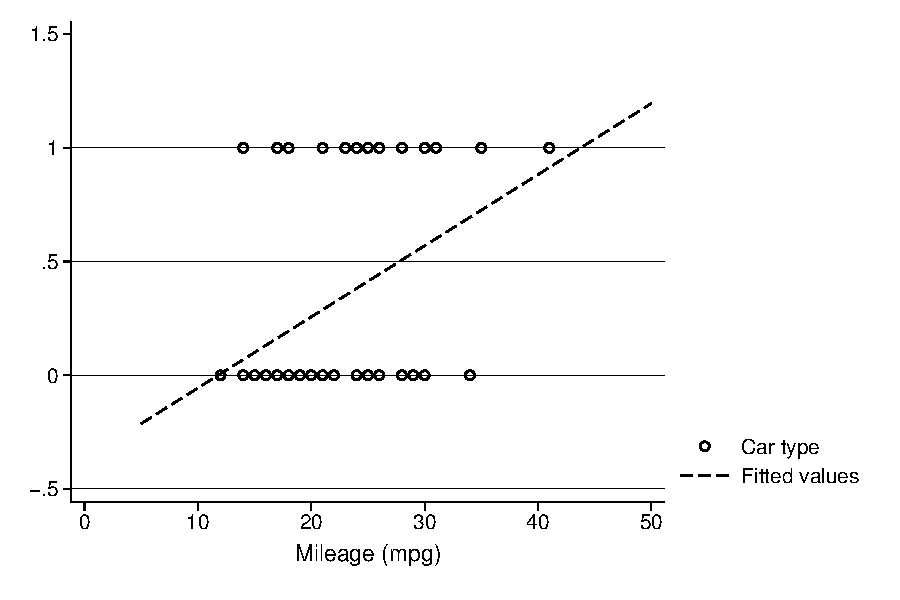
\includegraphics[width=\linewidth]{fig/mpl}
			\caption{Modelo de Probabilidad Lineal (MPL)}
			\label{img1}
		\end{minipage}
		\hfill
		\begin{minipage}{.48\linewidth}
			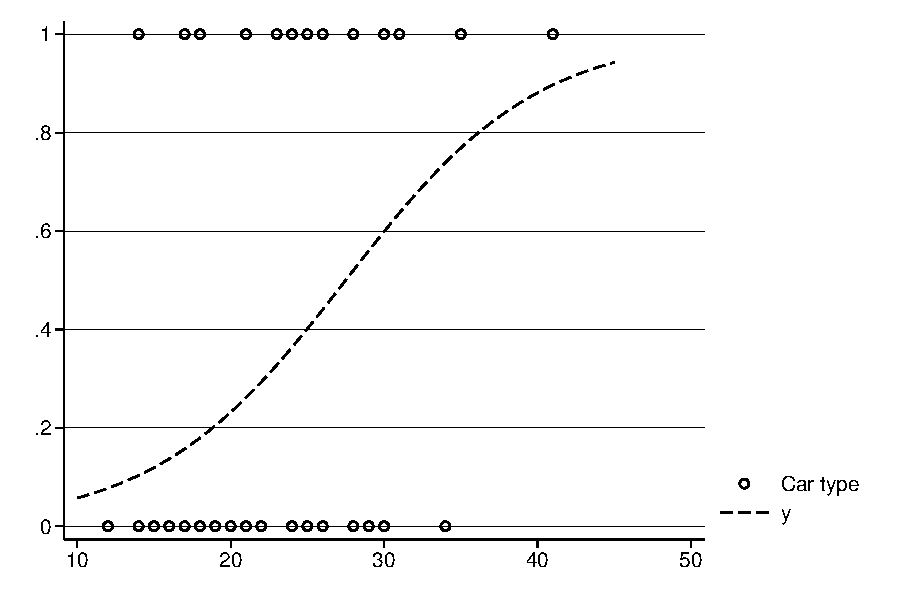
\includegraphics[width=\linewidth]{fig/mpnl}
			\caption{Modelo de Probabilidad No lineal}
			\label{img2}
		\end{minipage}
	\end{figure}
	
\end{frame}

\begin{frame}
	
	En teoría son varias las funciones no lineales que se
	pueden usar pero las mas populares son:
	\bigskip
	
	\begin{description}
		\item[Modelo Probit] $F(\omega)=\int_{-\infty}^{\omega}\frac{1}{\sqrt{2\pi}}e^{-t^2/2}dt$
		\item[Modelo Logit] $F(\omega)=L(\omega)=\frac{e^{\omega}}{1+e^{\omega}}$
	\end{description}
\end{frame}

\begin{frame}{Fundamento económico}
	Al menos dos justificaciones
	\begin{enumerate}
		\item Precio de reserva
		\item Modelo de utilidad aleatoria
	\end{enumerate}
\end{frame}


\subsubsection{Interpretación}

\begin{frame}{Efecto Marginal}
	
	El efecto marginal para la persona $i$ en la variable $k$, cuando
	la variable $x_k$ es continua se define como:
	
	\begin{eqnarray*}
		EM_{ik}=\frac{\partial Prob(Y_i=1)}{\partial x_k}=\frac{\partial F(X_i'\beta)}{\partial
			x_k}=\beta_k f(X_i'\beta)
	\end{eqnarray*}
	
	Mientras que cuando esta es dicotómica el efecto se define como:
	
	\begin{eqnarray*}
		EM_{ik}=F(X_i'\beta|x_k=1)-F(X_i'\beta|x_k=0)
	\end{eqnarray*}
\end{frame}

\begin{frame}{Comparación de Efectos Marginales}
	
	Una forma de comparar los resultados de los diferentes modelos es
	empleando efectos marginales:
	
	\begin{eqnarray}
		\frac{\partial}{\partial
			x_{ik}}x_i'\beta &=& \beta_k^{PL} \\
		\frac{\partial}{\partial x_{ik}}\Phi(x_i'\beta) &=& \phi(x_i'\beta)\cdot
		\beta_k^{Probit}\\
		\frac{\partial}{\partial x_{ik}}L(x_i'\beta) &=& \frac{e^{x_i'\beta}}{(1+e^{x_i'\beta})^2}\cdot
		\beta_k^{Logit}
	\end{eqnarray}
	
	Así, cuando $x_i'\beta=0$, se pueden tener ``equivalencias'' entre
	los distintos $\beta$s al igualar los efectos marginales de (1)
	con (2) y los efectos marginales de (1) y (3).
\end{frame}

\begin{frame}{Odds Ratios}
	
	En el caso de un logit del tipo:
	\begin{eqnarray}
		% \nonumber to remove numbering (before each equation)
		Pr[Y_j=1|X_j] &=& \frac{exp(\alpha_0+\beta_0 X_j)}{1+exp(\alpha_0+\beta_0 X_j)}
	\end{eqnarray}
	
	
	\textbf{Los odds} se definen como:
	
	\begin{eqnarray}
		Odds(X) &=& \frac{Pr[Y_j=1 | X_j]}{Pr[Y_j=0 | X_j]}=\frac{F(\alpha_0+\beta_0 X_j)}{1-F(\alpha_0+\beta_0
			X_j)}=exp(\alpha_0+\beta_0 X_j)
	\end{eqnarray}
	
	
	\textbf{Los odds ratios} es el ratio de dos odds para diferentes
	valores de $X_j$, digamos $X_j=x$ y $X_j=x+\Delta x$:
	
	\begin{eqnarray*}
		\frac{Odds(x+\Delta x)}{Odds(x)} &=& \frac{exp(\alpha+\beta x+\beta \Delta x)}{exp(\alpha+\beta
			x)}=exp(\beta \Delta x)
	\end{eqnarray*}
	
	%Tomando logaritmos...
\end{frame}


\subsection{Estimación}

\begin{frame}[fragile]
	\frametitle{Estimación}
	\begin{itemize}
		\item Se emplea MV
		
		\item Sea una muestra $y_1, y_2..., y_n$ cuya probabilidad de
		ocurrir es $P(muestra)$
		
		\item $P(muestra)=P(y_1)*P(y_2)*P(y_2)...*P(y_n)$, si cada
		$y_i$  es independiente
		
		\item Donde $P(y_i)=1-F(X_i\beta)$  si $y1=1$  o $P(y_i)=F(X_i\beta)$  si
		$y_i=0$
		
		\item La función de verosimilitud:
		\begin{eqnarray*}
			L &=& \Pi_{y_i=1}[1-F(-X_i\beta)]*\Pi_{y_i=0}F(-X_i\beta)
		\end{eqnarray*}
		
		\item Los $\beta$s los encontramos maximizando esta función
		(matemáticamente es un proceso iterativo, se empieza con un
		grupo de $\beta$s y se va iterando hasta alcanzar los $\beta$s óptimos)
	\end{itemize}
\end{frame}

%\subsection{Efectos Marginales}
%
%\begin{frame}[fragile]
%  \frametitle{Efectos Marginales}
%\begin{itemize}
%    \item La interpretación no es la misma que en un modelo lineal
%    
%    \item El impacto del las variables independientes (efecto marginal)
%     es diferente dependiendo del punto en el cual se calcula el impacto:
%    \begin{eqnarray*}
%      \frac{\partial F(X_i\beta)}{\partial x_{ik}} &=&
%      f(X_i\beta)\beta_k
%    \end{eqnarray*}
%    
%    \item Donde $f$ es la función de densidad de probabilidad (p.d.f)
%    
%    \item Puntos cercanos a la media tienen un impacto mucho mayor comparados con puntos en las `colas' de la distribución.
%\end{itemize}
%\end{frame}

\subsubsection{Logit nulo, ingenuo o baseline}

\begin{frame}[fragile]
	\frametitle{Modelo ingenuo}
	
	Estime el modelo logit ingenuo sabiendo que:
	\bigskip
	
	\begin{tabular}{c}
		% after \\: \hline or \cline{col1-col2} \cline{col3-col4} ...
		\hline
		Y \\
		\hline
		1 \\
		0 \\
		0 \\
		\hline
	\end{tabular}
\end{frame}

\subsubsection{Generalización}

\begin{frame}[fragile]
	\frametitle{Generalización}
	
	Sea $(y_i,x_i)$ con $i=1,...,n$, una muestra $iid$ $Y_i$ tiene una
	distribución de Bernoulli con $p_i=Pr(y_i=1)$ con lo cual la
	función de verosimilitud será:
	
	
	\begin{eqnarray*}
		L(\beta) &=& \prod_{y_i=1}p_i \prod_{y_i=0}(1-p_i)=\prod_{i=1}^n p_i^{y_i}(1-p_i)^{1-y_i}
	\end{eqnarray*}
	
	
	
	y su logaritmo:
	
	\begin{eqnarray*}
		l(\beta) &=& \sum_{i=1}^n [y_i (ln p_i)+(1-y_i)ln(1-p_i)] \\
		&=& \sum_{i=1}^n [y_i ln F(x_i'\beta)+(1-y_i)ln(1-F(x_i'\beta))]
	\end{eqnarray*}
	
\end{frame}

\begin{frame}[fragile]
	\frametitle{Generalización}
	
	Siendo las condiciones de primer orden:
	
	\begin{eqnarray*}
		\sum_{i=1}^n\frac{(y_i-F_i)f_i}{F_i(1-F_i)}x_{ki}&=&0
	\end{eqnarray*}
	
	con $k=1,...,K$; $F_i\equiv F(x_i'\beta)$ y $f_i\equiv
	f(x_i'\beta)$
	\smallskip
	
	
	
	En el caso particular de un logit
	$(F(x)=\frac{exp(x)}{1+exp(x)})$ la expresión se reduce a:
	
	\begin{eqnarray*}
		\frac{\partial \ln L}{\partial \theta }&=&\sum_{i=1}^{n}(y_{i}-F_i)\mathbf{x}%
		_{i}=\mathbf{0}
	\end{eqnarray*}
\end{frame}

\subsection{Curvas ROC}

\begin{frame}[fragile]
	\frametitle{Curvas ROC}
	\begin{itemize}
		\item  ¿Cómo predecir la ocurrencia de un evento a partir de la estimación de un modelo tipo probit
		o logit? (buen o mal pagador)
		\item Los modelos permiten calcular las probabilidades de
		ocurrencia, típicamente se asume que si la probabilidad predicha
		es superior a 0.5, entonces se asume que el evento ocurrirá.
		\item Reconocer que existen dos tipos de errores que se cometen cuando se
		hace la predicción discreta es la motivación de la estrategia
		ROC.
		\item El porcentaje de unos clasificados incorrectamente y el porcentaje de ceros clasificados
		incorrectamente se conocen como sensitividad y especificidad,
		respectivamente.
	\end{itemize}
\end{frame}

\begin{frame}[fragile]
	\frametitle{Curvas ROC}
	\begin{table}
		\centering
		\begin{tabular}{cccc}
			\hline \hline
			& \multicolumn{ 2}{c}{Verdadero} &            \\
			
			Clasificado &          D=1 &         D=0 &      Total \\
			\hline
			+ &          a &          c &        a+c \\
			
			- &          b &          d &        b+d \\
			\hline
			Total &        a+b &        c+d &    a+b+c+d \\
			\hline
		\end{tabular}
		\caption{Classified es $+$ si Pr(D) predicha $>=$ umbral}
	\end{table}
	
	Donde ``Verdadero'' hace referencia a lo efectivamente observado
	(lo verdadero), D=1 y ~D=0 y ``Classified'' es lo estimado
	probabilísticamente.
\end{frame}

\begin{frame}[fragile]
	\frametitle{Curvas ROC}
	Si la probabilidad de ocurrencia es mayor a un determinado umbral
	(por ejemplo $0.5$), entonces se clasifica como cierto la
	ocurrencia (+). A partir de lo predicho y lo efectivamente
	observado se pueden construir los siguientes indicadores:
	
	
	\begin{enumerate}
		\item \texttt{Sensitibidad:} Porcentaje de unos clasificados
		correctamente: $\frac{a}{a+b}$
		
		\item \texttt{Especificidad:} Porcentaje de ceros clasificados
		correctamente: $\frac{d}{c+d}$
		
		\item \texttt{Correctamente clasificados:} Total de correctamente clasificados: $\frac{a+d}{a+b+c+d}$
	\end{enumerate}
\end{frame}

\begin{frame}[fragile]
	\frametitle{Curvas ROC. Presentación gráfica}
	\begin{figure}
		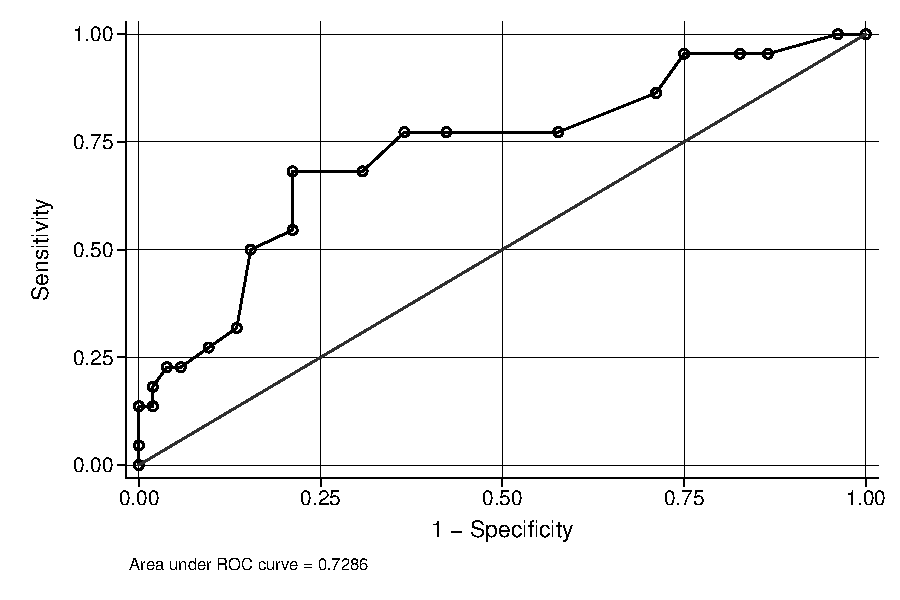
\includegraphics[scale=.6]{fig/lroc}
		\caption{Curva ROC.}
	\end{figure}
\end{frame}

\begin{frame}[fragile]
	\frametitle{Curvas ROC. Selección de modelos}
	
\end{frame}



\subsubsection{Evaluación del modelo}

\begin{frame}[fragile]
	\frametitle{Bondad de ajuste}
	\begin{itemize}
		\item Pseudo-R2 que compara la función de verosimilitud maximizada por nuestros betas con una función
		donde todos los betas son cero y solo hay una constante (modelo ingenuo)
		
		\item Formalmente: Test LR  (Likelihood ratio)
		
	\end{itemize}
\end{frame}
%3) Intervalos de confianza -------------------------------------------------
	%===============================================================================
\section{Interpretación}
%===============================================================================
\begin{frame}{Interpretación}
	\begin{itemize}
		\item $\hat{y}=\hat{\beta_{0}}+\hat\beta_{1}x_{1}+\hat\beta_{2}x_{2}+...+\hat\beta_{k}x_{k}$\\
		Tomando el operador diferencial:
		\item $\Delta\hat{y}=\hat\beta_{1}\Delta x_{1}+\hat\beta_{2}\Delta x_{2}+...+\hat\beta_{k}\Delta x_{k}$ \\
		Así, manteniendo fijos $x_{2},...,x_{k}$, entonces
		\item $\Delta\hat{y}=\hat{\beta_{1}}\Delta x_{1}$\\
		Interpretar
		\bigskip
		\begin{enumerate}
			\item $Ln(y)=\hat\beta_{0}+\hat\beta_{1} Ln(x_{1})$
			\item $Ln(y)=\hat\beta_{0}+\hat\beta_{1} x_{1}$
			\item $y=\hat{\beta_{0}}+\hat\beta_{1} Ln(x_{1})$
		\end{enumerate}
	\end{itemize}
\end{frame}

%4)Prueba de hipótesis sobre una combinación lineal simple de parámetros ----
	%====================================================================================
\section{Prueba de hipótesis sobre una combinación lineal simple de parámetros}
%====================================================================================

\begin{frame}{Medidas de Ajuste}
	Surgen algunas preguntas sobre el rendimiento del modelo.
		\begin{itemize}
			\item ¿Qué tan bien esa línea de regresión describe los datos?
			\item ¿Los regresores explican mucha o poca variación en la variable dependiente?
			\item ¿Están las observaciones dispersas o lejos de la línea de regresión?
		\end{itemize}
	El $R^2$ y el error estándar de la regresión miden qué tan bien la línea de regresión MCO $\ldots$ coincide con los datos. Estudiante: ¿Qué es el $R^2$?
		\begin{itemize}
			\item el $R^2$ mide la fracción de la varianza de $y$ que se explica por los regresores
			\item $0 < R^2 <1$
		\end{itemize}
\end{frame}
%---------------------------------------------------
\begin{frame}{Medidas de Ajuste}
	Consideremos el siguiente modelo
		$$Y_i = \widehat{Y}_i + \widehat{u}_i$$
	reexpresamos arriba en términos de varianza
		$$Var(Y_i) = Var	(\widehat{Y_i}) + Var(\widehat{u}_i)$$
	equivalentemente
		$$\frac{Var(\widehat{Y_i})}{Var(Y_i)} + \frac{Var(\widehat{u})}{Var(Y_i)} = 1$$
	o
		$$\frac{Var(\widehat{Y_i})}{Var(Y_i)} = 1 - \frac{Var(\widehat{u}_i)}{Var(Y_i)}$$
\end{frame}
%---------------------------------------------------
\begin{frame}{Medidas de Ajuste}
	Por lo tanto
		$$R^{2} = \frac{Var(\widehat{u}_i)}{Var(Y_i)} = 1 - \frac{SCR}{SCT}$$
	Ahora, necestimos definir la \textbf{Suma Cuadrado de la Regresión} (SCR) y \textbf{Suma Cuadrada del Total} (SCT).
		\begin{gather}
			SCT = \sum_{i=1}^{n}(Y_I-\overline{Y}_i)^2 \tag{SCT}\\
			SCR = \sum_{i^1}^{n}\widehat{\mu}_i^{2} \tag{SCR}
		\end{gather}
	Por lo tanto, si la varianza del error es igual a la varianza de $Y$, eso significa que nuestro modelo no tiene poder de predicción. Eso implica $R^{2} = 0$. Si nuestro modelo puede explicar la mayoría de los cambios de $y$, entonces $R^{2} \rightarrow 1$
\end{frame}
%---------------------------------------------------
\begin{frame}{Medidas de Ajuste: Ejemplo I}
	\begin{enumerate}
		\item En el ejemplo relativo a la estimación de una función de producción para Perú.
			$$Q=e^{\alpha_{0}}K^{\alpha_{k}}L^{\alpha_{l}}$$
		el $R ^ 2 = 0,80$. Eso significa que el 80\% de los cambios en la producción se deben a cambios en el capital y el trabajo.
		\item Tenemos los siguientes datos $y = [40\enskip 55\enskip 25\enskip 5\enskip 10]'$. Su querido profesor quiere que estimen el siguiente modelo $y_t = \beta_0+ u_t$ utilizando el estimador MCO. Específicamente;
			\begin{itemize}
				\item ¿Cuál es la estimación de $ \beta_0$
				\item ¿Cuál es el $R^2$?
			\end{itemize}
	\end{enumerate}
\end{frame}
%---------------------------------------------------
\begin{frame}{Medidas de Ajuste: Ejemplo II}
	\begin{enumerate}
		\item De las cuentas nacionales, tenemos la siguiente identidad $Y = C + I + G + XM$. Un estudiante que reprobó la econometría propuso el siguiente modelo para evaluar el impacto del consumo en el PIB ($Y$)
			$$Y_t = \beta_0+\beta_1C_t+\ldots +\beta_5M_t+u_t$$
			\begin{itemize}
				\item ¿Cuál es la media de $\widehat{u}^2$?
				\item ¿Cuál es el $R^2$?
			\end{itemize}
		\item el siguiente modelos
			\begin{align*}
				M_1 & : Y_i = \beta_0 + \beta_1X_{1i} + u_i\\
				M_2 & : Y_i = \gamma_0 + \gamma_1X_{1i} + \gamma_2X_{2i} + u_i
			\end{align*}
			El $R^2$ de $M_1$ y $M_2$ son 0.701 y 0.80 respectivamente.\\
			¿Qué modelo es mejor?
	\end{enumerate}
\end{frame}
%---------------------------------------------------
\begin{frame}{Una advertencia sobre R2}
	\begin{enumerate}
		\item El $R ^ 2$ aumenta cuando se agrega una nueva variable, por lo tanto, un aumento en el $R ^ 2$ no significa que agregar una nueva variable realmente mejora el ajuste del modelo.
		\item De hecho, aunque la nueva variable no es significativa, $R ^ 2$ aumenta.
		\item Un mal investigador puede inflar el ajuste del modelo agregando variables irrelevantes al modelo empírico.
		\item $R ^ 2$ es útil para mostrar el poder de explicación de su modelo, pero no para comparar.
	\end{enumerate}
\end{frame}
%---------------------------------------------------
\begin{frame}{Una alternativa: R2 ajustado o R2 adj}
	Tenemos una alternativa: el $R^2$ ajustado
		$$R^2 = 1 \frac{N - 1}{N - k} \frac{SCR}{SCT}$$
	Algunas observaciones sobre esta medida de ajuste o ajuste
		\begin{enumerate}
			\item El $R^2$-ajustado siempre es más bajo que $R^2$
			\item Agregar un regresor tiene dos efectos opuestos en $R^2$-ajustado
			\item El $R^2$-ajustado puede ser negativo
		\end{enumerate}
	Una advertencia con respecto a esta medida de ajuste.
		\begin{enumerate}
			\item La medida de $R^2$-ajustado aumenta (disminuye) cuando el cuadrado del valor $t$ realmente calculado, relacionado con la variable nueva o adicional, es mayor (menor) que uno.
			\item Al final, $R^2$-ajustado también es útil para mostrar el poder de explicación de su modelo y eso tiene cierto poder de comparación, pero también es débil.
		\end{enumerate}
\end{frame}
%5) Prueba de restricciones lineales múltiples: la prueba F -----------------
	%====================================================================================
\section[Censurado y truncado]{Modelos de regresión censurados y truncados}
%====================================================================================


\begin{frame}{A modo de repaso}
	\begin{itemize}
		\item Usamos probit y logit para una respuesta binaria.
		\item Usamos Tobit para una solución de esquina (``corner solution outcome'')   
	\end{itemize}
	Usualmente otro rasgo de los datos cae en la misma categor\'{i}a de variables restringidas por un valor; en este caso estamos hablando de una variable censurada.
\end{frame}
%---------------------------------------------------
\begin{frame}{El modelo de datos censurados}
	¿Cómo surge una variable censurada?
		\begin{itemize}
			\item \textit{Survey design}. Es un caso de missing data (en la variable dependiente). Por ejemplo, demanda por tickets en eliminatorias para los últimos cupos al mundial.
			\item En algunos casos restricciones institucionales (Wooldridge).	   
		\end{itemize}
\end{frame}
%---------------------------------------------------
\begin{frame}{El modelo de datos censurados}
	\begin{itemize}
		\item ¿Cúal es el rasgo del modelo de variable censurada? Las unidades son observables y proveen información de las variables independientes ($X$'s); pero la información sobre la variable dependiente esta ausente (variable omitida). Es de conocimiento el valor de corte. Este valor puede ser superior (\textit{right censoring}) o inferior (\textit{left censoring}).
		\item Unidades escogen opciones como ``mas de 50 000 dólares'' ( threshold); se observan datos menos de 50 000 dólares.
		\item La misma respuesta del \textit{threshold} para muchas observaciones $i$.
	\end{itemize}
\end{frame}
%---------------------------------------------------
\begin{frame}
	\begin{figure}[htbp]
		\hspace*{+1cm} 
		\centering
			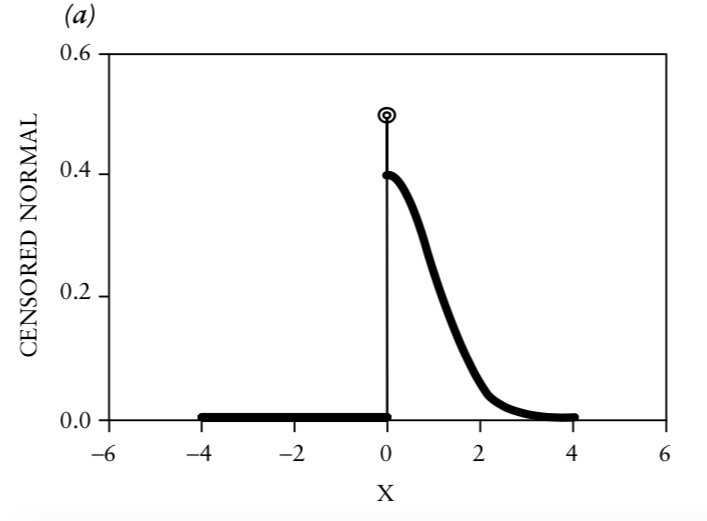
\includegraphics[width=0.65\linewidth]{fig/censored-model} % requires the graphicx package
		\label{censored}
		\caption{Source: Heij et. al 2004 ``Econometric Methods with Applications in Business and Economics''}
	\end{figure} 
\end{frame}
%---------------------------------------------------
\begin{frame}{El modelo de datos censurados}
	El modelo censurado puede expresarse de la siguiente manera:
		\begin{align}
			y_i=& \boldsymbol{x_i\beta}+u_i, \ u_i |  \ x_i, c_i \ \sim Normal(0,\sigma^2) \\
			w_i=&\min(y_i,c_i)
		\end{align}
	$u_i$ is independent of $c_i$
\end{frame}
%---------------------------------------------------
\begin{frame}
	¿Cuál es el problema de estimar este modelo por OLS? Las razones son similares como en el caso del modelo TOBIT.
		\begin{itemize}
			\item Los $\beta$'s son inconsistentes.	
		\end{itemize}
	Sin embargo existe un punto importante; en el modelo TOBIT, se esta modelando comportamiento óptimo de los individuos ($y\equiv$ consumo de alcohol), y en el modelo censurado se tiene un problema en el método de recolección porque (por alguna razón) una porción de los datos son censurados (no observados).
\end{frame}
%---------------------------------------------------
\begin{frame}{El modelo de datos censurados}
	Exploremos la siguiente base de datos en la página de \href{http://fmwww.bc.edu/ec-p/data/wooldridge/datasets.list.html}{\textcolor{cyan}{Wooldridge}}. Utilizar el siguientes comando ``bcuse recid''. Una descripción de las variables en la siguiente figura:
	\begin{figure}[htbp]
		\hspace*{+1cm} 
		\centering
			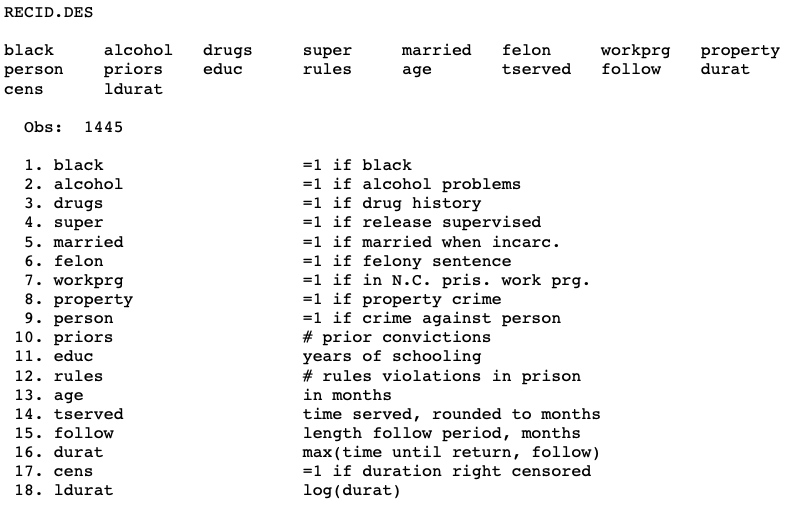
\includegraphics[width=0.53\linewidth]{fig/recid} % requires the graphicx package
		\label{recid}
		\caption{recid.des in Wooldridge's datasets}
	\end{figure} 
\end{frame}
%---------------------------------------------------
\begin{frame}{El modelo de datos truncados}
	\begin{itemize}
		\item Un modelo de datos censurados es aplicable cuando se tiene observaciones de las unidades y la información es parcial; es decir, se tiene información de las variables independientes pero no de la variable $y$.
		\item Usamos Tobit para una solución de esquina (``corner solution outcome'').
		\item Un modelo truncado tiene la característica de excluir (basado en el valor de $y$ ). No se tiene una submuestra aleatoria. Sin embargo, tenemos conocimiento de la regla de exclusión. Esta regla esta determinada si $y$ esta por encima o por debajo de cierto valor (o ``threshold'').   
	\end{itemize}
\end{frame}
%---------------------------------------------------
\begin{frame}{El modelo de datos truncados}
	?`Como surge o se identifica un modelo de datos truncados?
		\begin{itemize}
			\item El investigador presta atención a una submuestra de la población (quizas debido a costos de muestreo, ver Wooldridge). 		   
			\item Hay que enfatizar que la estimación por OLS es eficiente cuando la muestra seleccionada es aleatoria.
		\end{itemize}
	Ejemplos: Hausman y White (1977) usan data de impuestos negativos a la renta como determinante  de las ganancias individuales/familiares. El estudio solo incluía familias con renta 1.5 veces la linea de pobreza.
\end{frame}
%---------------------------------------------------
\begin{frame}{El modelo de datos truncados}
	El modelo de datos truncados puede expresarse de la siguiente manera;
		\begin{equation}
			y=\boldsymbol{x\beta}+u, u \ | \ x, \ \sim Normal(0,\sigma^2)
		\end{equation}
	y el set de datos ($y,x$) es observado solo si $y\ge c_i$ donde el ``threshold'' depende de variables x. Por ejemplo, Haussman y white (1977) definen $c_i$ como el tama\~no de la familia.  
\end{frame}
%---------------------------------------------------
\begin{frame}
	La funcion de distribución gráficamente luce de la siguiente manera;
		\begin{figure}[htbp]
			\hspace*{+1cm} 
			\centering
				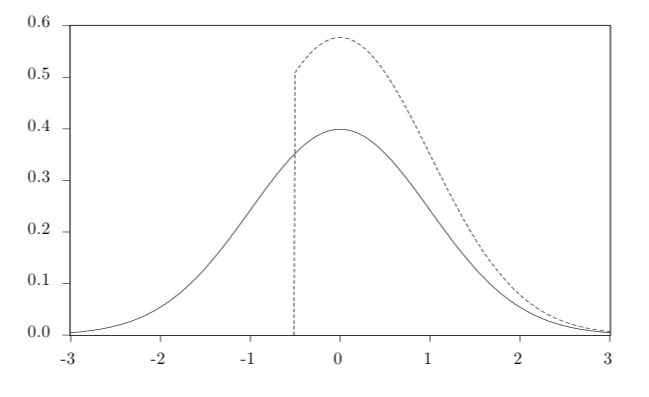
\includegraphics[width=0.70\linewidth]{fig/truncated-model} % requires the graphicx package
			\label{trunc}
			\caption{Source: Chumacero, R, 2003: ``Limited dependent variable'' handout}
		\end{figure} 
\end{frame}
%---------------------------------------------------
\begin{frame}{El modelo de datos truncados}
	La funcion de distribución formalmente luce de la siguiente manera;
		\begin{align}
			g(y|x_i,c_i)=&f(y|x_i\beta,\sigma^2)/F(c_i|x_i,\beta,\sigma^2), y\le c_i
		\end{align}
	donde $f(y|x_i\beta,\sigma^2)$ denota la función de densidad normal y $F(c_i|x_i,\beta,\sigma^2)$ es la función acumulada evaluada en el threshold $c_i$.
	En pocas palabras, se re-pondera dividiendo la función de densidad normal por la acumulada para que la nueva función de densidad sume el valor de uno (1) sobre el dominio de los datos.
	Luego, se toman logs y se estima por ML (es decir, se maximiza la función ($g(y|x_i,c_i$) con los datos observados).
\end{frame}
%---------------------------------------------------
\begin{frame}{!`Vayamos a STATA!}
	Tengamos en cuenta un estudio que tiene el objetivo de modelar el desempe\`no académico como una función de las destrezas de lenguaje (``language skills'') y el tipo de programa en el que los estudiantes se han matriculado. Se requiere analizar a los estudiantes que tengan un desempe\~no mínimo de 40. Tengamos en cuenta la siguiente base de datos en formato STATA:
	\\
	use https://stats.idre.ucla.edu/stat/stata/dae/truncreg, clear
\end{frame}


%6) Informe de resultados de regresión --------------------------------------
	%====================================================================================
\section{Importando datos}
%====================================================================================

\begin{frame}[fragile]{Importando datos}
	Importamos datos f�cilmente a STATA. Tengamos la siguiente sintaxis
		$$\cdot\enskip \textup{\texttt{use \textcolor{blue}{\textit{filename}} [, clear nolabel]}}$$
	no olvides \colorbox{codegray}{\texttt{help import}} para comprobar la sintaxis. Aqu� algunos ejemplos
\begin{lstlisting}[language=Stata, numbers=none]
use "http://wps.aw.com/wps/media/objects/
11422/11696965/empirical/empex_tb/cps92_08.dta"
use auto, clear
webuse lifeexp, clear
\end{lstlisting}
\end{frame}

%---------------------------------------------------
\begin{frame}[fragile]{Otros formatos: XLS, XLSX y CSV}
	Importamos f�cilmente datos a STATA desde otros formatos. Tengamos la siguiente sintaxis
		$$\cdot\enskip \textup{\texttt{import \underline{exc}el [using] \textcolor{blue}{\textit{filename}} [, \textcolor{blue}{\textit{import\_excel\_options}}]}}$$
	no olvides \colorbox{codegray}{\texttt{help import}} para comprobar la sintaxis. Aqu� algunos ejemplos
\begin{lstlisting}[language=Stata, numbers=none]
import exc using grades_data.xlsx, first clear
insheet using grades_data.csv, clear
\end{lstlisting}
	no olvides \colorbox{codegray}{\texttt{help insheet}} para comprobar la sintaxis entera.
\end{frame}
%----------------------------------------------------------------------------
	\note[itemize]{
		\item Agregar alguna nota
	}

%------------------------------------------------------------------------------------
% End
%----
	\begin{frame}
		\maketitle
	\end{frame}
%------------------------------------------------------------------------------------
\end{document}		
%====================================================================================